\chapter{Implementation}
%% & Testing
%% This is the chapter in which you review the implementation and testing
%% decisions and issues, and critique these processes.

\newlist{requirementsrevisit}{enumerate}{1}
\setlist[requirementsrevisit]{label=\textbf{R\arabic{subsection}.\arabic*}}

\section{Introduction}
Throughout this chapter, we divulge and explain the third party software and toolset we used to implement the system.
We also look to describe problems faced along the way, and the proposed solutions to those problems. 
It is important to notice that not all issues are included: trivial or academically uninteresting problems are ignored in favour of those more interesting and relevant. 
An assumption is made that the reader has a working knowledge of web development throughout this chapter.


\section{Base Technologies}
\subsection{Clientside Technologies}
In section \ref{littechconclusion}, it was decided that the system should be a website based application, and we desire it so that users can access the system independent of browser, operating system or device.
It was felt that developing and testing for the top three most used browsers, as reported by w3schools.com (http://www.w3schools.com/browsers/browsers\_stats.asp) would cover adequate scope for the timeline of this project, and further browser testing and tweaking will be left for future work. 
Thus, the browsers chosen were Google Chrome, Firefox and Safari.

In order to achieve this browser-agnostic system, we built the website using standard web technologies, specifically HTML5, CSS3 and JavaScript.
These languages enable a page to provide content, styling and interaction, respectively.
The goal was to ensure that the code would work well across browsers and operating systems, with small, trivial adaptations applied in specific circumstances.
Due to limited time for this project, it was decided to focus on the release of each browser with the highest percentage of users in the month that testing began (February 2016), as reported by w3schools.com (http://www.w3schools.com/browsers/browsers\_stats.asp). 
This amounted to the versions C48 for Google Chrome, FF 44 for Firefox and S 9 for Safari.
The system was also developed to run on an iPad and iPhone, to get as close to a device-agnostic system as time and resources allowed. Further devices are left to future work.

Further to this, all code was run through the W3C compliant check to ensure the code is compliant with web standards.
Having standardised code provides a degree of confidence that the website will function correctly as browsers update, or in different browsers not yet tested.

All of this together resulted in a base system that users can visit and navigate, though no interaction was possible, due to no memory or state change within the system.
In order to achieve this, database and serverside technologies are required, to communicate between the database, the web server and the client's browser, providing the degree of state change we require.
Figure \ref{homepage} shows the design of the homepage, with placeholder data, which will later be served by the serverside technologies.

\begin{figure}[htb!]
  \centering
  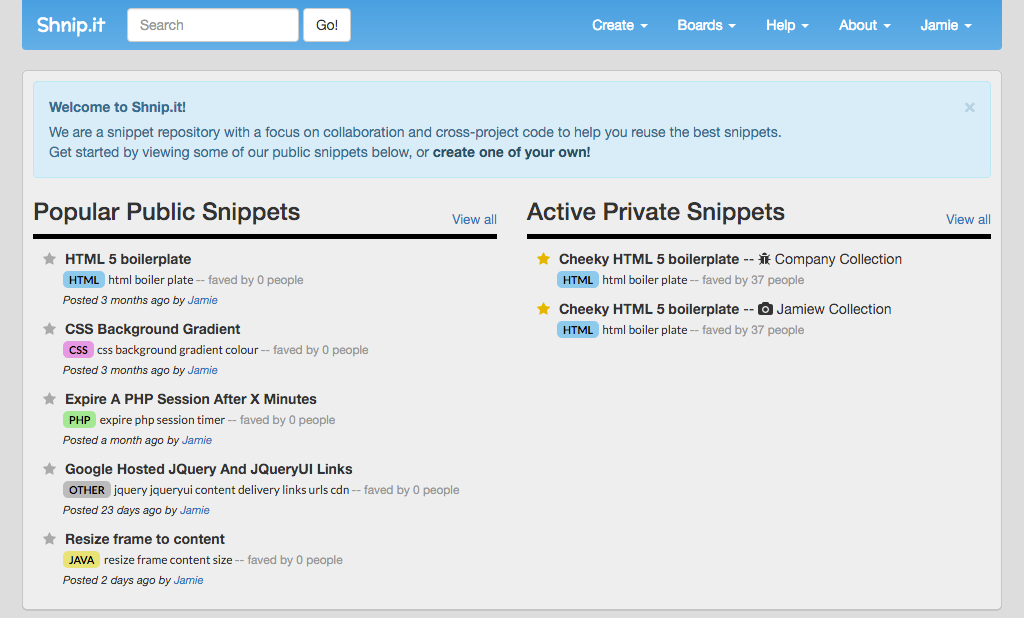
\includegraphics[scale=0.4]{homepage}
  \caption{Shnip.It's Home Page \label{homepage}}
\end{figure}

\subsection{Serverside Technologies}
The chosen technologies for the serverside are PHP and MYSQL, due in part to the authors experience with them, and the fact that, as a pair, they are well known in industry.
PHP is parsed before the webpage is sent to the client, and the output of any PHP process is plain HTML that can then be sent to the web browser for viewing.
This provides an efficient method of querying the database to retrieve information depending on which page the user wished to view, and then providing that page with the appropriate content filled in via PHP.
PHP is also used to handle the majority of website functionality, including account registering/login, the editing and saving of snippets, and all other information related to the usage of the website.

We also use a MYSQL database as it provides a relational structure suited to the envisioned structure of the website. 
The interaction between PHP and MYSQL is well-structured and documented, allowing for easier development of the website's backend.
Finally, a visual representation of the database is provided via a tool named PHPMYADMIN, which is accessible from the server's IP, as seen in Figure \ref{phpmyadmin}.
This technology is useful for quickly creating the database, and managing it visually.

\begin{figure}[htb!]
  \centering
  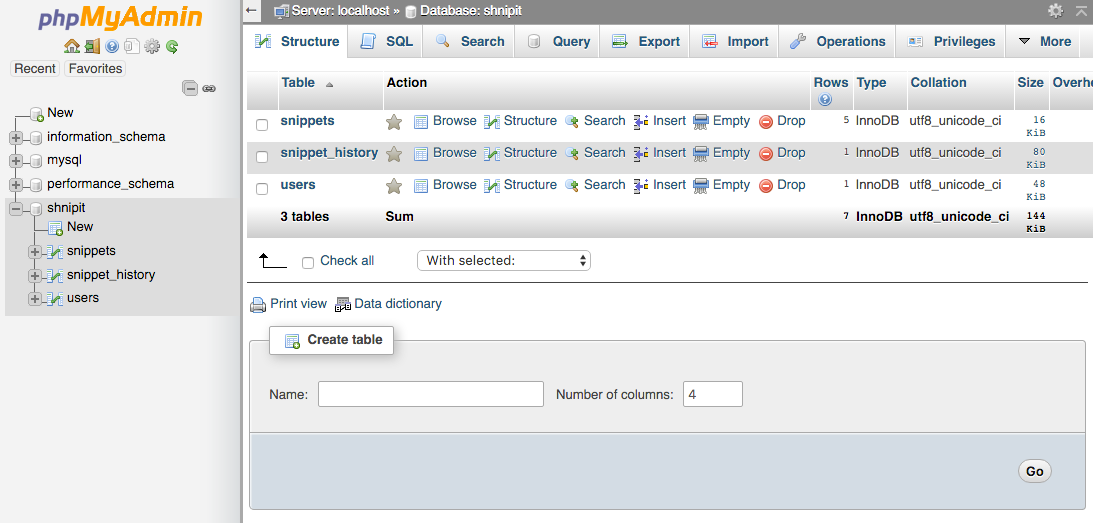
\includegraphics[scale=0.3]{phpmyadmin}
  \caption{Shnip It database structure, visualised in PHPMYADMIN \label{phpmyadmin}}
\end{figure}

\section{External Plugins \& Libraries}
\subsection{Environment Libraries}
A number of external plugins were utilised within the development environment, either as a way to write better code or to promote the cross-compatibility of the code across browsers.
The first of these technologies was named SASS, and the second, its counterpart Compass. 

SASS is a precursor language that converts its markup into valid CSS, while providing the user with functionality not available with standard CSS.
Such functionality includes variables, for example hexidecimal colour codes, that can be reused throughout the SASS and easily changed, or mixins that allow code to be written once and reused throughout. 
This enables a more object oriented style of CSS to be written, and cuts down on development time, both initially and in the future when the design may change.
Furthermore, Compass is used as a utility that converts these SASS files to CSS files on the fly, and allows the developer to forget about the conversion process.

Finally, a stylesheet named Normalise.css was utilised which resets a number of styles that may differ by default between different browsers, for example margins or padding on specific elements.
It was used to give a more consistent baseline between browsers, so that less minor tweaks were required further down the line.

\subsection{Development Libraries}
A number of development libraries were used, either to provide functionality that had already been created, or to use as a method of writing less code.

Bootstrap is the first library used; it offers a styling baseline for the website, including dynamic grids that can adjust easily to screen size, certain pre-created elements such as notifications, widgets and buttons, and a general, good practice environment from which to build upon.

JQuery was utilised to make page-specific Javascript easier to perform. 
The design involved interaction between the user and the page, such as rating a snippet or submitting a comment; as such, jQuery allowed for more effective and efficient interaction, by providing immediate confirmation of a successful action, as opposed to refreshing the page to show the updated content.
Examples of these are showing the comment on screen, or colouring in an up arrow for a positive rating. 

Finally, we used a number of libraries that had been created to do specific tasks, rather than re-writing them. 
This included Prism to handle the syntax highlighting, an optional feature noted in section \ref{optionalfeatures}, Moment maker to make `fuzzy timestamps' such as 3 hours ago, and identicon to create unique default profile pictures based on a user-centric alphanumeric string. 
All 3 of these libraries can be seen in Figure \ref{snippetpage}.
These are all libraries to handle optional features that were included in the final system.

\begin{figure}[htb!]
  \centering
  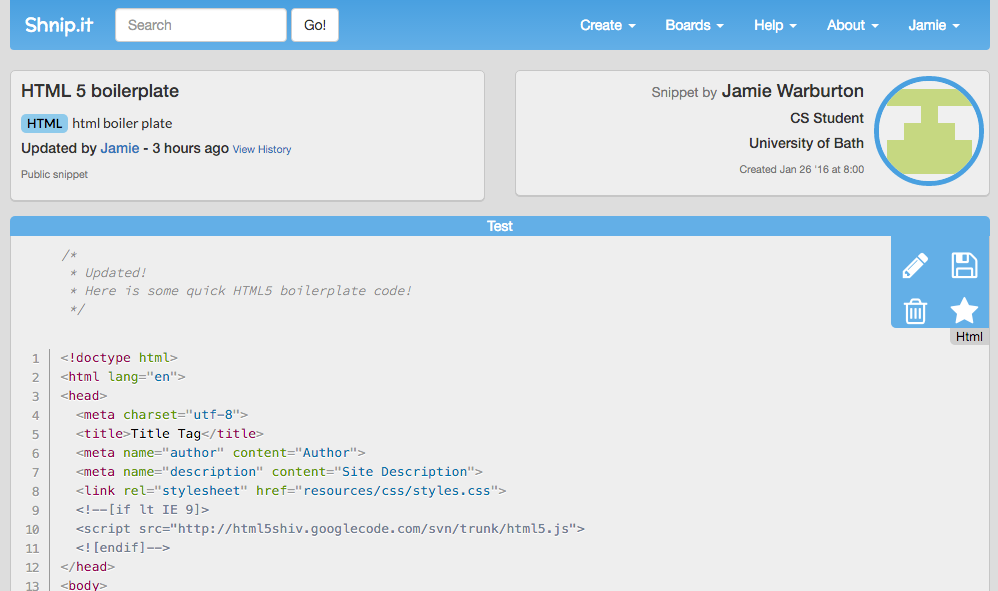
\includegraphics[scale=0.4]{snippetpage}
  \caption{Snippet Page - Syntax Highlighting, and `3 hours ago' fuzzy timestamp \& Identicon \label{snippetpage}}
\end{figure}

\section{Novel Problems}

\subsection{Database Design and Access}

A key component of our system was the database, as it would hold the entire catalogue of the website; without it the website would not function.
This meant it was important to design it to be efficient, robust and secure. 

\subsubsection{Designing the Database}
Due to the nature of how accounts and snippets are linked, a decision was made to build a relational database, enabling a table per element, and to link them via IDs.
However, this posed two novel problems - how would we calculate, store and retrieve the number of upvotes and downvotes a specific post has received - and by whom - and also how to handle the version history and control of snippets, specifically in relation to snippet collections.

\subsubsection{Upvotes and Downvotes}
There are two obvious approaches to this problem: \\
	1. Create a table for upvotes and downvotes, and attribute each vote to a snippet ID, and a user ID, and calculate the total when required, or \\
	2. Ignore the normalisation of the database, and just store a total in the snippet table for each snippet, and increment or decrement as required.

Both of these methods suffer from some form of scalability issue. 
For the first approach, recalculating would have to be performed every time the value of the total number of votes was required, which can equate to several times per page refresh, or many tens of times per homepage refresh, due to these pages showing information for more than one snippet.
Multiplied by the number of users active and this can become quite the computationally expensive solution.

The second method opts to store the total in the table with the snippet, and so cuts out a significant portion of the computation originally suggested.
However, with this solution, the total can easily fall out of sync with reality, as parallel writes to the database may conflict or not be recorded, and the database may spend a considerable portion of time trying to ensure that increments and decrements were not overwriting each other, and attempting to maintain an accurate record.
In practice, this equates to a slow, inaccurate database. This problem is further compounded by the fact that there is no record of who has voted, and so no method of preventing a user from voting multiple times.

After some research into this issue, it was decided to follow a pattern similar to that of Stack Overflow's, which is a hybrid of the two solutions above. 
Initially, we store a total value within the snippets table, and ignore the normalisation exclusively for this field.
We also keep a separate table consisting of snippet ID, user ID and the vote value (1 or negative 1). 
When we need to display the total value of all votes, we simply query the snippet table and receive the total as listed, which solves our expensive computation problem on reading the total.

Next, when a specific action occurs, such as a user up or down-voting a snippet, the system records the vote in the correct table, then recalculates the total value of that snippet, and updates the snippet table. 
This solution avoids the out-of-sync problems faced, while also providing a record of who has voted, and as reading the total is much more common than writing it, the expensive computation on reading the total is ultimately reduced, and in turn significantly lowering the computational cost of the overall solution.

\subsection{Version History}
The next issue we encountered was related to storing the version history for each snippet in an efficient manner.
At first this does not seem like a trivial problem, however it was confounded by the inclusion of `grouped snippets' - that is, groups of snippets that go together, for example a snippet of HTML, one of CSS and one of JavaScript that collectively describe a button.

Initially we had a single table of all snippets, each having an ID and a date. 
These two fields together allowed us to describe a unique snippet, with all historical versions having the same ID but a different date.

However, this resulted in duplication of static data, such as original author and date of creation, amongst other fields.
To remove this redundant data, a two table design was utilised - one to parent the snippets, which has a single row per snippet, and one to contain the historical data for the snippets.
The two tables were linked by a field named `child snippet', which stored the ID of the historical snippet, and functioned identically to the original design in the previous paragraph.

This worked well until the inclusion of grouped snippets, as a method of tracking the parent snippet, as well as all the children snippets, was required.
A simple solution would have been to create another table of a similar design, which would be the parent of the grouped snippets, and would store the IDs of the static snippets, which in turn hold the IDs of the versioned snippets.
It is easy to see this design is cumbersome and could quickly become a burden, and so a different solution was required.

We already had the static snippet table functioning as a parent for the version history snippets, so felt it was natural to extend this.
We opened up the `child snippet' field to accept an array of IDs, and so it became `child snippets'.
This structure can be seen in Figure \ref{tablelayout}.
Now we were able to track all of the child snippets, but it left us with a number of questions surrounding how to treat each snippet in terms of interaction - should they have their own rating systems, or collectively for the entire snippet group?

\begin{figure}[htb!]
  \centering
  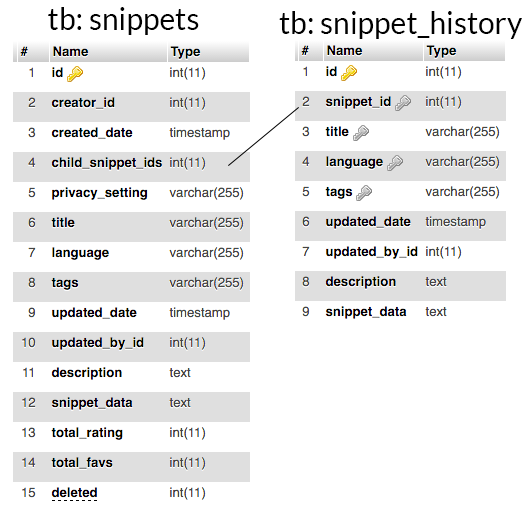
\includegraphics[scale=0.6]{tablelayout}
  \caption{Database Structure - Grouped Snippets \label{tablelayout}}
\end{figure}

For the purpose of this dissertation, each group was treated as a single snippet, and were given a single, overall rating system. We leave it for future work to research and conclude the preferable method for this.

\subsection{Database Security} \label{DBSec}
For the website to function, the database must hold user information and passwords, and therefore must be secure.
It is of great importance to endeavour to follow best practices surrounding this sensitive data and the storage of it, therefore research into this area was required.

We began with the most obvious - account information, and specifically the passwords. 
As we are using PHP, the best practices for password storage were researched, and it was decided to use PHPs built in password hashing functions. 
With this, PHP handles the password hashing and checking, and allows us to simply store the hashed string in our database for later comparison.
As PHP updates, so too do the functions, and as such the system is given an evolving method of security with little cost to development or maintenance.

Next we turned to the security of the database itself. 
Initially the user accounts that login to the database were considered, and these were given complex passwords, particularly for the root users, to help prevent brute force attacks on the database itself.
The user permissions were also cleaned up to ensure only necessary permissions were given to each of the user accounts.

Last on the list was the code. 
Initially we made sure that only the web server had access to any files that contain database login information, so they couldn't simply be found and viewed outside of the web server. 
Then the interaction with the database was examined, via SQL.
This is important due to a method of hacking called SQL injection.
While there exist a number of methods to prevent this, such as prepared statements, it was decided instead to use an external library, called Medoo.

Medoo is a lightweight PHP database framework, built by developers more versed in database design and security than the authors of this dissertation.
Medoo allows us to call simple functions to interact with the database, while maintaining the full security of more complex code, as Medoo wraps this code for us.
The end result is relatively simple interaction code for us to write, without having to worry about security every time we write this code.
A final benefit of Medoo is similar to that of PHP - the code is updated to include any new security features, but our code remains the same, so maintaining the website is less troublesome.
Sample code for inserting data into the database via Medoo can be found in Appendix \ref{medoocode}.


%% What users can access - Groups, private boards, private group boards etc

\section{Summary} \label{implementsummary}

\subsection{Revisiting the Requirements} \label{requirementsrevisited}

We now revisit our list of requirements and discuss how well we have delivered upon them:

\subsection{Delivery on Non-functional Requirements}
\textbf{These Requirements had a high priority}

\begin{requirementsrevisit}

    \item Security \label{security} \\
	\textit{Our system is in line with current best practices, and employs the use of libraries that can easily be updated to incorporate updated security without code changes. Passwords are only stored as hashes via approved methods, private files are only accessible by the web server, and all database user passwords and permissions are set appropriately.}

    \item Ease of Use \label{easeofuse} \\
	\textit{This will be ascertained throughout the course of the evaluation. However, the system has a clear design with obvious icons to indicate functionality and so should be sufficient.}

    \item Simple and Clear \label{simpleandclear} \\
	\textit{This, too, shall be ascertained throughout the evaluation. Again, the clear design and obvious icons should help alleviate mistakes.}

    \item Memorability \label{memorability} \\
	\textit{The simplistic nature of the website combined with the minimal number of pages should allow users to easily re-establish proficiency in use.}

    \item Familiarity \label{familiarity} \\
	\textit{The website uses standard icons for particular functions, as well as obvious styling for elements such as buttons, links and interactive elements.}

    \item Self Policing \label{selfpolicing} \\
	\textit{The system enables users to vote up and down snippets, and uses these votes to automatically police the content via hiding it if it goes too low, and prominently displaying the higher rated snippets. The system also enables users to comment their opinions, and submit edit requests to improve the code.}

Overall we feel our high priority Non-Functional requirements were met well.

\end{requirementsrevisit}

\textbf{These Requirements had a low priority}

\begin{requirementsrevisit}[resume]

    \item Open Source \label{opensource} \\
	\textit{The system currently is not open source, however this is a simple change to make which we leave to future work.}

Overall our low priority Non-Functional requirement was not met, though it is left for future work.

\end{requirementsrevisit}


\subsection{Delivery on Functional Requirements}
\textbf{These Requirements had a high priority}

\begin{requirementsrevisit}

    \item History \label{history} \\
	\textit{The system keeps track of all additions/changes/deletions made, in completion, within the database.}

    \item Accountability \label{accountability} \\
	\textit{The system stores the user ID alongside all additions/changes/deletions to attribute them to that user.}

    \item Social Activity \label{socialactivity} \\
	\textit{The system provides comments, ratings, favouriting and edit requests to allow interaction, both user-to-user and user-to-snippet.}

    \item Content Navigation/Discovery \label{content} \\
	\textit{While a high priority requirement for our system, this is thought to be out of scope for the purposes of this dissertation. Instead, a minimal search function was implemented, to allow users to navigate and discover content, though advanced search is left for future work.}

    \item Privacy \label{privacy} \\
	\textit{The system provides the ability to set snippets to public, private or accessible by a set of email addresses. Accounts with those email addresses attached are then able to view the content.}

    \item Password Security \label{passwordsecurity} \\
	\textit{The system uses PHP's built in functions to hash passwords, and allows these functions to easily update with appropriate advances in the technology.}

    \item Data Security \label{datasecurity} \\
	\textit{All unauthorised material is hidden by a login authentication wall. Some of the website is accessible without an account, but interaction requires login and authentication.}

    \item Platform Compatible \label{platformcompatible} \\
	\textit{The system works appropriately on the latest versions of Google Chrome, FireFox and Safari, on both Windows 7/8/10 and Mac OS X El Capitan. It also works appropriately on iPhone and iPad with Google Chrome and Safari.}

Overall, the majority of our high priority Functional requirements were met, with the exclusion of complex search and sort. However, this requirement was deemed out of the scope of this dissertation, and so was left for future work.

   \end{requirementsrevisit}

\textbf{These Requirements had a low priority}

\begin{requirementsrevisit}[resume]

    \item Gamification \label{gamification} \\
	\textit{The system as of yet does not employ gamification - however we leave it to future work to implement points for positive submissions, and achievements for completing particular milestones, which can be shown on your profile and be made public.}

    \item Submission Groups \label{submissiongroups} \\
	\textit{Snippets can be combined into snippet groups, allowing for multiple snippets to be treated as one singular snippet, for example HTML, CSS and JavaScript snippets that are grouped and describe a singular button.}

While we achieved one of the low priority Functional requirements, we didn't include gamification. It was decided that this will be left for future work, but plans for how to proceed were decided already.

\end{requirementsrevisit}


These will be evaluated further in the evaluation chapter of this dissertation, however, as the majority of the requirements were met, we can expect a satisfactory solution.

\section{Conclusion}
Throughout this chapter it was shown that the implementation of our system has met almost all of the high priority requirements, with the exception of one deemed out of scope of this dissertation. 
We have also discussed novel issues faced throughout the implementation and the solutions chosen to overcome them.
The next chapter describes the user studies we performed to evaluate our system.

